
\documentclass[12pt]{article}

\usepackage[margin=1in]{geometry}
\usepackage{amsmath, amssymb, amsthm}
\usepackage{newtxtext,newtxmath}
\usepackage[scaled=0.92]{helvet}
\usepackage[T1]{fontenc}
\usepackage{graphicx}
\usepackage{booktabs}
\usepackage{hyperref}
\hypersetup{
  colorlinks = true,
  linkcolor  = black,
  citecolor  = black,
  urlcolor   = blue,
  pdfborder  = {0 0 0},
}
\usepackage[numbers,sort&compress]{natbib}
\usepackage[dvipsnames,table]{xcolor}
\usepackage{lineno}
\usepackage{setspace}
\usepackage{algorithm}
\usepackage{algpseudocode}
\usepackage{titlesec}
\usepackage{enumitem}

\usepackage{caption}
\renewcommand{\figurename}{Fig.}
\captionsetup{labelsep=space, labelfont=bf, font=small}

\setlength{\parindent}{0pt}
\setlength{\parskip}{0.35em}
\renewcommand{\arraystretch}{1.2}

\titleformat{\section}
{\large\bfseries}
{\thesection}
{0.75em}
{}

\titleformat{\subsection}
{\normalsize\bfseries}
{\thesubsection}
{0.75em}
{}

\setlist[itemize]{leftmargin=1.5em,itemsep=0.15em,topsep=0.15em}
\setlist[enumerate]{leftmargin=1.5em,itemsep=0.15em,topsep=0.15em}

\linenumbers
\doublespacing

\newcommand{\TODO}[1]{\par\medskip\noindent
  \begingroup\color{red}\textbf{[\,EMMANUEL:\;} #1 \textbf{]}\endgroup
  \par\medskip}
\newcommand{\TODOi}[1]{\begingroup\color{red}\textbf{[\,EMMANUEL:\;} #1 \textbf{]}\endgroup}

\newtheorem{theorem}{Theorem}
\newtheorem{proposition}{Proposition}
\newtheorem{remark}{Remark}

\begin{document}

% ============================================================
% TITLE PAGE  (MBEC requires a separate title page carrying:
% title; author names/affiliations; corresponding author
% contact; total manuscript word count; abstract word count;
% figure count; table count.)
% ============================================================
\begin{titlepage}
\thispagestyle{empty}

\begin{center}
{\LARGE\bfseries When Inverse Physics-Informed Neural Networks
Become Practically Identifiable: A Case Study in Synaptic
Dopamine Transport \par}
\end{center}

\vspace{1.5em}
\noindent Emmanuel Hackman\textsuperscript{1,*} \quad
Huiqing Zhu\textsuperscript{1}

\vspace{0.5em}
\noindent\textsuperscript{1}School of Mathematics and Natural
Sciences, University of Southern Mississippi, Hattiesburg,
MS 39406, USA

\vspace{0.5em}
\noindent\textsuperscript{*}Corresponding author:
Emmanuel Hackman \\
E-mail: \texttt{Emmanuel.Hackman@usm.edu} \\
Telephone: +1 (601) 266-4934 (School of Mathematics and Natural
Sciences office) \\
Fax: Not applicable

\vspace{1.5em}
\noindent\textbf{Manuscript counts} \\
Total word count (title page through Conclusion, excluding
Declarations and reference list): approximately 7{,}200 \\
Abstract word count: 198 \\
Number of figures: 4 \\
Number of tables: 5

\vspace{1.5em}
\noindent\textbf{Author biographies} \\[0.5em]
Emmanuel Hackman is with the School of Mathematics and Natural
Sciences, University of Southern Mississippi, working on
physics-informed machine learning methods for inverse problems
in biomedical transport modeling.
\TODOi{Verify/expand: add your degree program and level (e.g.
``PhD candidate in...''), and trim to $\leq$200 characters
including spaces. Optional photo.} \\[0.5em]
Huiqing Zhu is with the School of Mathematics and Natural
Sciences, University of Southern Mississippi.
\TODOi{Co-author to supply: title/degree, research focus, and
trim to $\leq$200 characters. Optional photo.}

\end{titlepage}

\newpage
\noindent\textbf{Keywords:} Physics-informed neural networks;
dopamine diffusion; reaction-diffusion equations; inverse
problem; Parkinson's disease
\TODO{Springer MBEC asks for keywords preferably drawn from the
MeSH database -- ``Parkinson Disease'' and ``Dopamine'' are
exact MeSH terms; ``physics-informed neural networks,''
``reaction-diffusion equations,'' and ``inverse problem'' are
not MeSH terms as such -- consider whether closer MeSH matches
(e.g. ``Neural Networks, Computer''; ``Synaptic Transmission'')
should replace them before submission.}

\begin{abstract}

Quantifying dopamine clearance matters for understanding
dopaminergic dysfunction in Parkinson's disease, but classical
mesh-based inversion struggles under sparse, noisy observations
typical of experimental recordings. We formulate recovery of
the diffusion coefficient $D$ and reuptake rate $k$ as a
parameter inverse problem for a 2D reaction-diffusion PDE of
synaptic dopamine transport, using physics-informed neural
networks (PINNs) as a mesh-free forward and inverse solver. All
validation uses synthetic data from a finite-difference
reference; no biological measurements are used yet. The forward
model attains an L2 relative error of $1.52\%$ against the
finite-difference reference and $3.75\%$ against the analytical
solution. For the
inverse problem, evaluated over a five-seed ensemble, we recover
$D = 0.3515 \pm 0.0034$ $\mu\text{m}^2/\text{ms}$ and
$k = 0.0573 \pm 0.0006$ $\text{ms}^{-1}$, with mean relative
errors of $9.85\%$ and $14.61\%$. The inverse problem is
well-conditioned along one direction and ill-conditioned along
a diffusion-reuptake trade ray, with implications for real-data
experimental design. Unlike a Levenberg-Marquardt baseline,
which drives $k$ to non-physical negative values under
bounded-domain data, the PINN's residual-based formulation
recovers physically meaningful parameters. This
identifiability-aware framework is a reusable tool for
inverse-PDE recovery of synaptic neurotransmitter dynamics;
application to experimental fast-scan cyclic voltammetry data
is the immediate next step.

\end{abstract}

\section*{Glossary of Terms}
\label{sec:glossary}

\begin{tabular}{@{}lll@{}}
$C(x,y,t)$ & dopamine concentration field & $\mu$M \\
$D$        & effective diffusion coefficient & $\mu\text{m}^2/\text{ms}$ \\
$k$        & linearised DAT reuptake rate constant & $\text{ms}^{-1}$ \\
$L$        & domain side length & $\mu$m \\
$T$        & simulation time window & ms \\
$\sigma$   & release-pulse half-width & $\mu$m \\
$C_0$      & peak release concentration & $\mu$M \\
\end{tabular}

\section{Introduction}
\label{sec:intro}

Parkinson's disease (PD) is the second most prevalent
neurodegenerative disorder worldwide, affecting approximately
10 million people and imposing a substantial public-health
burden \cite{GBD2016}. Its hallmark pathology is progressive
degeneration of dopaminergic neurons in the substantia nigra
pars compacta, reducing dopamine availability in the striatum
and producing the cardinal motor symptoms of PD: bradykinesia,
rigidity, and tremor \cite{Hornykiewicz1966, DeLong2007}.

Dopaminergic signaling begins when an action potential triggers
$\text{Ca}^{2+}$-dependent vesicle fusion, releasing
$\sim$$10^3$--$10^4$ dopamine molecules into the
$\sim$20\,nm synaptic cleft~\cite{Wiencke2020}. Released
dopamine diffuses through the cleft and surrounding
extracellular space with an effective diffusion coefficient
$D \approx 0.3\,\mu\text{m}^2/\text{ms}$~\cite{Nicholson1981,
CraggRice2004}, while clearance is mediated by the dopamine
transporter (DAT), modeled at sub-saturating concentrations as
a first-order reuptake rate $k$~\cite{CraggRice2004}. PD reduces
both the density of functional release sites and total striatal
DAT expression~\cite{Rice2008, CraggRice2004}, so changes in the
effective $(D, k)$ pair are a quantitatively meaningful proxy for
disease state. Fast-scan cyclic voltammetry (FSCV) provides
millisecond-resolution, sub-micrometer dopamine recordings
\emph{in vivo} and \emph{ex vivo}~\cite{Rodeberg2017}, but
yields exactly the sparse, noisy observation regime in which
recovering $(D, k)$ is hardest.

Classical reaction-diffusion models of dopamine transport
\cite{Nicholson1981, Rice2008, Wiencke2020} use finite-difference
or finite-element solvers, which require costly mesh construction
in complex neuroanatomical geometries and repeated forward solves
inside optimization loops for parameter estimation -- an approach
that scales poorly and is ill-suited to sparse experimental data.
Physics-informed neural networks (PINNs)~\cite{Raissi2019}
instead embed the governing PDE directly into the network's
training objective, solving forward and inverse problems on a
mesh-free domain. PINNs have been applied to cardiac
electrophysiology~\cite{Sahli2020}, systems-biology reaction
kinetics~\cite{Yazdani2020}, and PDE discovery from neural
imaging~\cite{Rudy2017}, but, to the best of our knowledge and
conditional on the limits of our literature search, have not
previously been applied to synaptic neurotransmitter diffusion.

This paper makes four contributions. First, we present an
inverse-PINN formulation for the spatially-resolved 2D
reaction-diffusion dynamics of synaptic dopamine transport,
extending prior inverse-PINN work in systems
biology~\cite{Yazdani2020} -- which addressed lumped ODE
kinetics without spatial structure -- to a spatially explicit
neurotransmitter transport problem. Second, we validate the
forward solver against both a closed-form analytical solution
and a finite-difference reference, showing the PINN attains
relative $L^2$ errors comparable to established numerical
schemes without a spatial mesh. Third, we solve the
corresponding inverse problem, recovering $D$ and $k$ from
sparse, noisy synthetic observations, and characterize its
practical identifiability: the problem is well-conditioned
along one direction and ill-conditioned along a
diffusion-reuptake trade ray, with direct implications for
experimental design. We further show that the PINN's
bounded-domain residual formulation succeeds where a classical
Levenberg-Marquardt baseline fails, driving $k$ to non-physical
negative values under the same data. Fourth, we release the
complete implementation -- seed-controlled training scripts and
a reproducible notebook -- as an open-source artifact, providing
a ready-to-extend baseline for sensitivity analysis and for
application to experimental FSCV data, which we identify as the
immediate next step toward a patient-specific tool for assessing
dopaminergic dysfunction in PD.

\section{Methods}
\label{sec:methods}

\subsection{Model Formulation}
\label{sec:math}

We model the spatiotemporal evolution of dopamine concentration
$C(x, y, t)$ on a two-dimensional spatial domain spanning the
synaptic cleft and the immediately surrounding perisynaptic
extracellular space, with axes $(x, y)$ in the plane parallel
to the pre- and postsynaptic membranes. The 2D restriction is
motivated by three factors: the cleft is geometrically thin
($h \approx 20$--$30\,\text{nm}$ normal to the membranes, two
orders of magnitude below the lateral spreading scale
$\sqrt{2DT} \approx 3.6\,\mu\text{m}$), so vertical equilibration
is essentially instantaneous and the in-plane distribution
captures the dynamics of interest; prior computational treatments
of striatal dopamine kinetics, most directly Wiencke et
al.~\cite{Wiencke2020}, adopt the same abstraction; and the 2D
problem admits a closed-form analytical reference solution
(Online Resource 2) for forward-solver validation. Extension to
3D perisynaptic geometries is a straightforward modification of
the input layer and PDE residual, identified as future work
(Section~\ref{sec:disc_future}).

Following Cragg
and Rice~\cite{CraggRice2004}, we approximate the action of
the dopamine transporter at sub-saturating concentrations by a
first-order linear sink $-k\,C$; this linearization is accurate
when $C \ll K_m$ (where $K_m$ is the Michaelis constant of DAT,
$\sim$0.2\,$\mu$M) and reduces the parameter-recovery problem
to two scalars $(D, k)$. The dopamine release event is modeled
as a radially symmetric Gaussian spatial pulse imposed at
$t = 0$ rather than as a sustained source, consistent with the
sub-millisecond timescale of vesicular
exocytosis~\cite{Wiencke2020}.

With these modeling choices, we consider the reaction-diffusion
initial-boundary-value problem on the square domain
$\Omega = (-L/2, L/2)^2$, $t \in (0, T]$,

\begin{equation}
  \frac{\partial C}{\partial t} = D\,\nabla^2 C \;-\; k\,C,
  \quad (x, y) \in \Omega,\ t \in (0, T],
  \label{eq:pde}
\end{equation}
where $\nabla^2 C = \partial_{xx} C + \partial_{yy} C$ is the
two-dimensional Laplacian, with the radially symmetric Gaussian
initial condition

\begin{equation}
  C(x, y, 0) = C_0 \exp\!\left( -\frac{x^2 + y^2}{2\sigma^2} \right),
  \quad (x, y) \in \overline{\Omega},
  \label{eq:ic}
\end{equation}

and zero-flux (Neumann) boundary conditions on all four edges
of $\partial \Omega$,
\begin{align}
  \left.\frac{\partial C}{\partial x}\right|_{x=\pm L/2}
    &= 0, \quad y \in [-L/2, L/2],\ t \in (0, T],
    \label{eq:bc_left} \\
  \left.\frac{\partial C}{\partial y}\right|_{y=\pm L/2}
    &= 0, \quad x \in [-L/2, L/2],\ t \in (0, T].
    \label{eq:bc_right}
\end{align}

The zero-flux conditions \eqref{eq:bc_left}--\eqref{eq:bc_right}
encode chemical isolation from neighboring synaptic compartments
on the timescales of interest -- either boundaries placed far
enough that the field has decayed to negligible amplitude by
$T$, or the symmetry of a periodic release-site
array~\cite{Wiencke2020}. The Gaussian profile in \eqref{eq:ic}
represents the instantaneous spatial footprint of a single
quantal release event, with $\sigma$ the effective release
radius and $C_0$ the peak concentration, decoupling the fast
release biophysics from the slower diffusion and reuptake
dynamics that are the focus of this study.

All model parameters are taken from the experimental dopamine
literature for striatal tissue~\cite{CraggRice2004, Nicholson1981}
and are summarized in Table~\ref{tab:params}.

\begin{table}[h!]
\centering
\caption{\textbf{Model parameters for the dopamine synaptic
diffusion problem.} Diffusion coefficient $D$ and
reuptake rate $k$ are taken from canonical experimental
values for striatal tissue; domain length $L$, release width
$\sigma$, and peak release concentration $C_0$ are taken
from the Wiencke et al.~\cite{Wiencke2020} computational
model. Simulation time $T$ is a modelling choice covering
the post-release diffusion window without significant
boundary interaction.}
\label{tab:params}
\begin{tabular}{llll}
\toprule
\textbf{Parameter} & \textbf{Symbol} & \textbf{Value} & \textbf{Source} \\
\midrule
Diffusion coefficient    & $D$   & $0.32$ $\mu\text{m}^2/\text{ms}$ & \cite{Nicholson1981, CraggRice2004} \\
Reuptake rate constant   & $k$   & $0.05$ $\text{ms}^{-1}$           & \cite{CraggRice2004} \\
Domain length            & $L$   & $5.0$ $\mu\text{m}$               & \cite{Wiencke2020} \\
Simulation time          & $T$   & $20$ ms                            & (model choice) \\
Peak source amplitude    & $C_0$ & $1.0$ $\mu$M                       & \cite{Wiencke2020} \\
\bottomrule
\end{tabular}
\end{table}

\subsection{Implementation and Reproducibility}
\label{sec:implementation}

Detailed JAX/Flax NNX code listings for the network module, PDE
residual, and inverse-problem training loop are provided in
Online Resource 1; the closed-form analytical solution
derivation underlying the forward-problem validation reference
is provided in Online Resource 2.

\begin{figure}[h!]
  \centering
  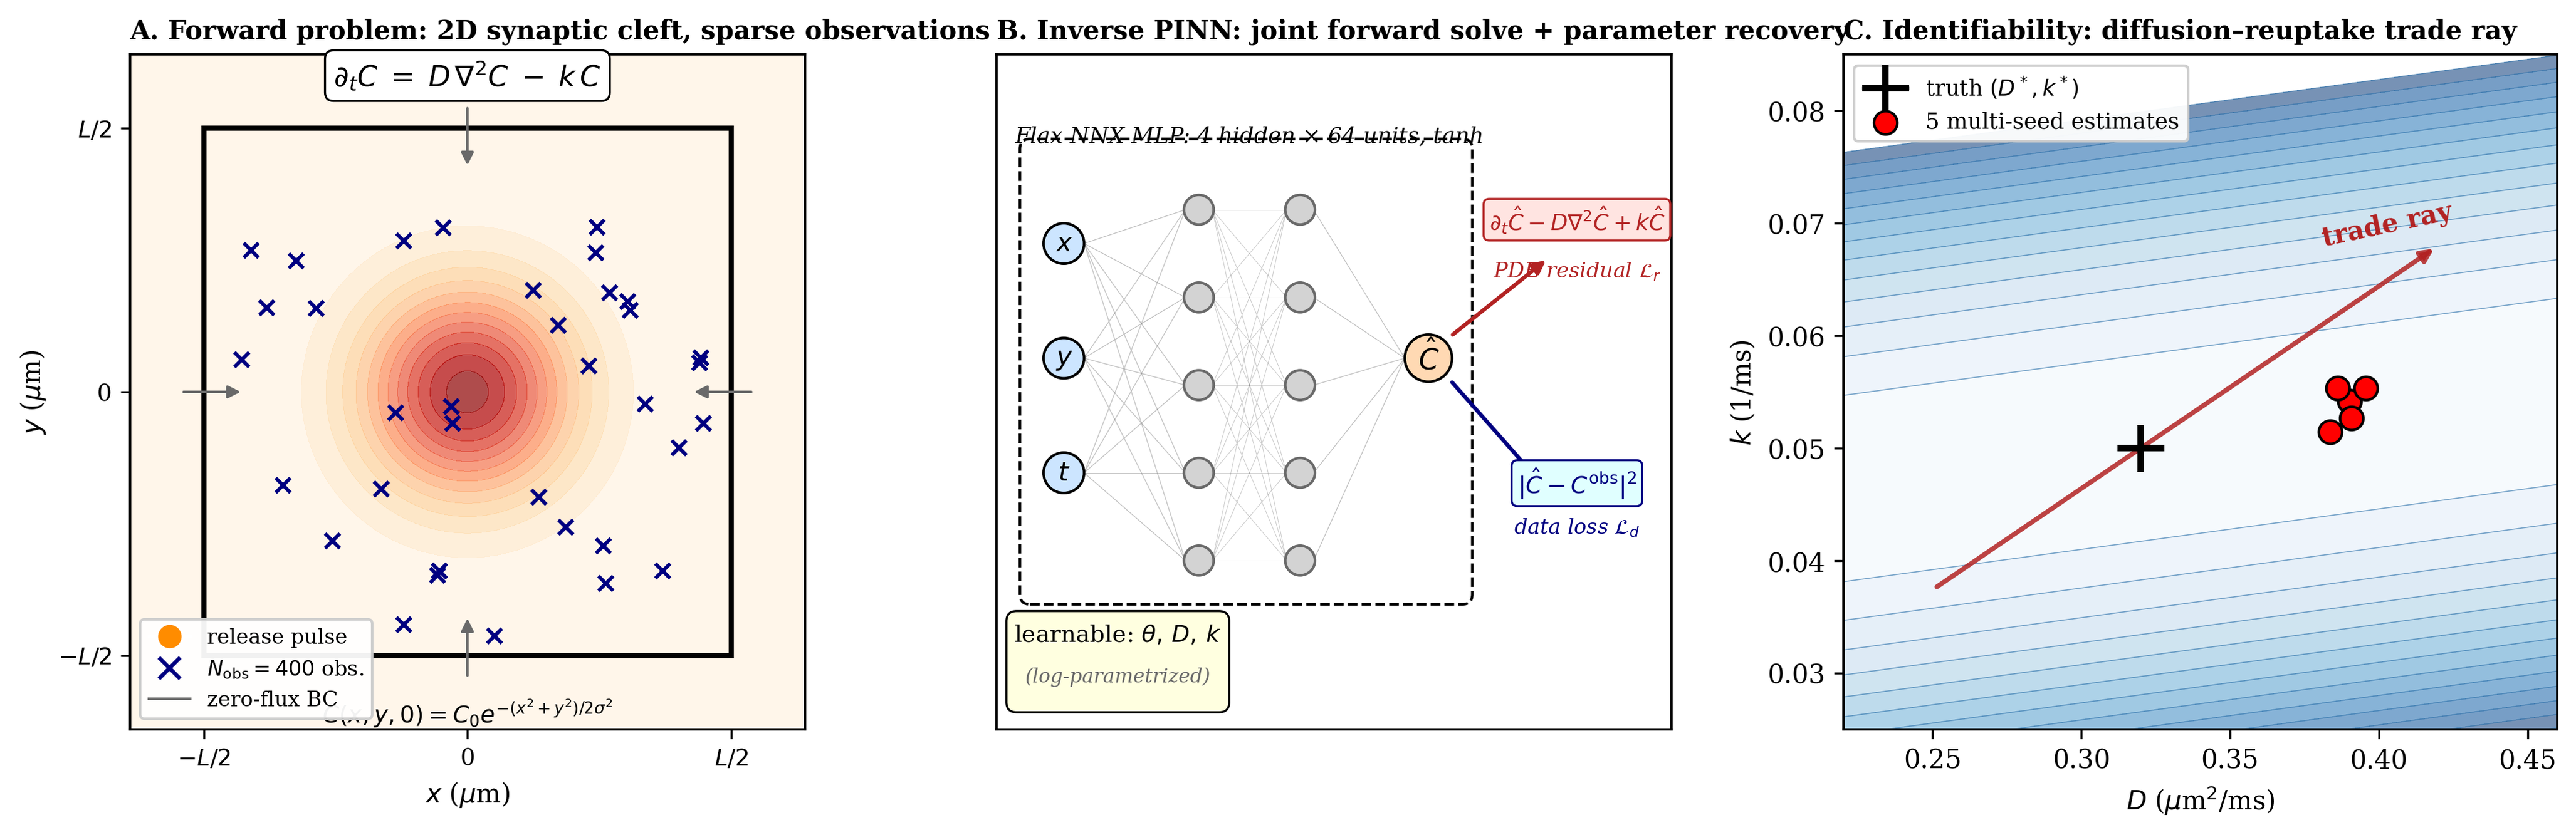
\includegraphics[width=0.98\textwidth]{../02_Figures/Fig1_preview.png}
  \caption{\textbf{Overview of the inverse-PDE problem and the
  physics-informed neural network methodology.}
  \textbf{A.} Forward setting: dopamine diffusion governed by a 2D
  reaction-diffusion PDE on the square synaptic domain
  $\Omega = [-L/2, L/2]^2$ with zero-flux Neumann boundary
  conditions and a radially symmetric Gaussian release pulse
  centred at the origin. Crosses mark a representative subset of
  the $N_{\mathrm{obs}} = 400$ sparse noisy observations used by the
  inverse problem.
  \textbf{B.} Inverse PINN methodology: a Flax NNX MLP
  $\mathcal{N}_\theta : (x, y, t) \in \mathbb{R}^3 \mapsto
  \hat{C} \in \mathbb{R}$ is trained to satisfy the PDE residual
  (red box) at $N_r$ interior collocation points while also
  fitting the sparse noisy observations through the data loss
  (blue box). The diffusion coefficient $D$ and the reuptake
  rate $k$ are exposed as log-parametrized learnable scalars and
  are optimized jointly with the network weights, so a single
  training run recovers both the concentration field and the
  underlying PDE parameters.
  \textbf{C.} Identifiability: the inverse problem exhibits a
  one-dimensional ``trade ray'' through $(D, k)$ space along
  which the loss landscape is flat to within the noise scale.
  Five network-initialization seeds (red dots) converge to
  estimates that cluster along this ridge above the ground-truth
  $(D^*, k^*) = (0.32, 0.05)$, reflecting the structural
  identifiability limit characterised in
  Section~\ref{sec:identifiability} rather than a
  finite-sample artefact}
  \label{fig:schematic}
\end{figure}

\subsection{PINN Architecture}
\label{sec:arch}

We employ a fully-connected feedforward neural network
$\mathcal{N}_\theta : \mathbb{R}^3 \to \mathbb{R}$,
parameterized by trainable weights and biases $\theta$, that
takes as input the space-time coordinates $(x, y, t)$ and
outputs the predicted dopamine concentration
$\hat{C}(x, y, t; \theta)$.

The network comprises four hidden layers of $64$ neurons each
with $\tanh$ activation (continuously differentiable, the
standard PINN choice~\cite{Raissi2019}):
\begin{equation}
  \hat{C} = \mathcal{N}_\theta(x, y, t) =
  (W_\ell \circ \sigma \circ W_{\ell-1} \circ \cdots
  \circ \sigma \circ W_1)(x, y, t),
  \label{eq:network}
\end{equation}
with $\ell = 5$ weight matrices (four hidden layers plus a
linear output layer, allowing $\hat{C}$ unbounded range). Weights
use Glorot initialization~\cite{Glorot2010}; the network has
$12{,}801$ trainable parameters in total.

Spatial and temporal derivatives in the PDE residual
\eqref{eq:pde} are evaluated by automatic differentiation of
$\mathcal{N}_\theta$, removing any need for finite-difference
stencils. The implementation uses JAX~\cite{JAX2018} with the
network as a Flax NNX module~\cite{Heek2020}, Adam via
Optax~\cite{Optax2020}, and L-BFGS via
jaxopt~\cite{Blondel2022}; JIT compilation gives a
2--5$\times$ speed-up over a comparable PyTorch implementation.
Complete source code and seed-controlled training scripts are
publicly available (Declarations: Code availability).

\subsection{Loss Function Formulation}
\label{sec:loss}

The total PINN loss function is the weighted sum of four terms:
\begin{equation}
  \mathcal{L}(\theta) = \lambda_r \mathcal{L}_r
  + \lambda_i \mathcal{L}_i
  + \lambda_b \mathcal{L}_b
  + \lambda_d \mathcal{L}_d,
  \label{eq:loss_total}
\end{equation}
The scalar weights $\lambda_r, \lambda_i, \lambda_b, \lambda_d \ge 0$
control the relative contribution of each term; imbalanced
weights induce gradient pathologies that prevent
convergence~\cite{Wang2021}. The individual terms are defined
as follows.

\paragraph{Residual loss $\mathcal{L}_r$} enforces the PDE
at $N_r$ collocation points
$\{(x_j^r, y_j^r, t_j^r)\}_{j=1}^{N_r}$:
\begin{equation}
  \mathcal{L}_r = \frac{1}{N_r} \sum_{j=1}^{N_r}
  \left| \frac{\partial \hat{C}}{\partial t}\bigg|_j
  - D\,\nabla^2 \hat{C}\bigg|_j
  + k\,\hat{C}_j \right|^2.
  \label{eq:loss_r}
\end{equation}

\paragraph{Initial condition loss $\mathcal{L}_i$} at
$N_i$ points:
\begin{equation}
  \mathcal{L}_i = \frac{1}{N_i} \sum_{j=1}^{N_i}
  \left| \hat{C}(x_j^i, y_j^i, 0) - C_0(x_j^i, y_j^i) \right|^2.
  \label{eq:loss_i}
\end{equation}

\paragraph{Boundary condition loss $\mathcal{L}_b$} at
$N_b$ boundary points:
\begin{equation}
  \mathcal{L}_b = \frac{1}{N_b} \sum_{j=1}^{N_b}
  \left| \mathcal{B}[\hat{C}](x_j^b, y_j^b, t_j^b) \right|^2,
  \label{eq:loss_b}
\end{equation}
where $\mathcal{B}[\cdot]$ denotes the boundary condition
operator corresponding to \eqref{eq:bc_left}--\eqref{eq:bc_right}.

\paragraph{Data loss $\mathcal{L}_d$} (for inverse problem;
set $\lambda_d = 0$ for forward problem) at $N_d$ observation
points:
\begin{equation}
  \mathcal{L}_d = \frac{1}{N_d} \sum_{j=1}^{N_d}
  \left| \hat{C}(x_j^d, y_j^d, t_j^d) - C_j^{\text{obs}} \right|^2.
  \label{eq:loss_d}
\end{equation}

We upweight the PDE residual relative to the other terms,
using $(\lambda_r, \lambda_i, \lambda_b) = (10, 1, 1)$ for the
forward problem ($\lambda_d = 0$) and
$(\lambda_r, \lambda_i, \lambda_b, \lambda_d) = (10, 1, 1, 1)$
for the inverse problem, keeping the residual on the same
gradient scale as the other terms and, in the inverse case,
preventing the optimizer from fitting observations at the
expense of physical consistency. Weights are held fixed
throughout training; adaptive schemes such as NTK-based
reweighting~\cite{Wang2021} are not used here and are
identified as future work.

\subsection{Collocation Point Sampling}
\label{sec:sampling}

Collocation points are sampled from the three-dimensional
space-time domain $\Omega \times (0, T]$ using Latin Hypercube
Sampling (LHS), which provides better coverage than uniform
random sampling~\cite{McKay1979}. Specifically, we use
$N_r = 10{,}000$ interior collocation points, $N_i = 400$
initial-condition points sampled uniformly over $\Omega$, and
$N_b = 400$ boundary points distributed across the four edges
of $\partial \Omega$ ($100$ per edge). An additional $5{,}000$
points are reserved as a held-out test set for monitoring
generalization during training. All samples are regenerated
from a fixed random seed at the start of each run to ensure
reproducibility.

\subsection{Training Procedure}
\label{sec:training}

Training proceeds in two phases: Adam~\cite{Kingma2015} for
$20{,}000$ iterations at fixed learning rate $10^{-3}$, followed
by limited-memory BFGS~\cite{Liu1989} via
jaxopt~\cite{Blondel2022} to convergence (max.\ $5{,}000$
iterations, gradient tolerance $10^{-9}$), exploiting
second-order curvature once iterates enter a local minimum's
neighborhood. Loss weights follow Section~\ref{sec:loss} and
are held fixed throughout; adaptive reweighting
schemes~\cite{Wang2021} are left for future work.

All experiments use a fixed random seed (1234), so re-runs
reproduce results to within floating-point tolerance. End-to-end
forward-problem training completes in $3$--$5$ minutes on a
single NVIDIA T4 GPU ($10$--$15$ minutes on CPU); the complete
reproduction pipeline (forward training, validation against both
references, the five-seed inverse ensemble, and figure
generation) completes in $\sim 50$ minutes on a T4 GPU, aided by
JIT compilation of the training step (a $2$--$5\times$
speed-up over a comparable PyTorch implementation; see Online
Resource 1 for implementation detail).

\subsection{Inverse Problem Formulation}
\label{sec:inverse}

The forward problem of Section~\ref{sec:math} assumes $D$ and
$k$ are known and seeks $C(x,t)$ satisfying
\eqref{eq:pde}--\eqref{eq:bc_right}. In the inverse setting
these roles reverse: given a partial, noisy observation of the
concentration field, we recover $(D, k)$. Such problems are
expensive for classical mesh-based solvers, since each candidate
$(D, k)$ requires a separate nested forward solve, with cost
growing linearly in the number of candidates~\cite{Wiencke2020}.
PINNs sidestep this nesting by treating $D$ and $k$ as
additional trainable parameters of the same network, so a
single training run recovers both the concentration field and
the physics constants~\cite{Raissi2019, Haghighat2021}.

Synthetic observations
$\{(x_j^d, y_j^d, t_j^d, C_j^{\text{obs}})\}_{j=1}^{N_d}$ are
generated by sampling locations uniformly from
$\Omega \times [t_{\min}, t_{\max}]$ with $t_{\min} = 0.5\,$ms
(just past the initial-condition transient, so data carry
information about both $D$ and $k$) and
$t_{\max} = 0.9\,T = 18\,$ms (the window over which the pulse
remains well-confined; cf.\ Online Resource 2). At each
location, the true concentration is computed by interpolating
the finite-difference reference solver (at $D=D^*$, $k=k^*$)
and corrupted by additive Gaussian noise,
\begin{equation}
  C_j^{\text{obs}} = C^*(x_j^d, y_j^d, t_j^d) + \varepsilon_j,
  \quad \varepsilon_j \sim \mathcal{N}\!\left(0,\,(\eta\, C_0)^2\right),
  \label{eq:observation}
\end{equation}
with $\eta$ the noise level as a fraction of $C_0$. Using the
finite-difference (rather than analytical) reference keeps the
observations exactly consistent with the Neumann boundary
conditions enforced by the PINN, avoiding a data-model mismatch
that would otherwise bias recovery at large $t$. Unless stated
otherwise, $N_d = 400$ and $\eta = 0.02$ ($2\%$, comparable to
high-quality FSCV noise floors~\cite{Rodeberg2017}).

$D$ and $k$ are introduced as trainable variables in the same
back-propagation graph as $\theta$, parametrized in log space
($D = \exp(\tilde{D})$, $k = \exp(\tilde{k})$) to enforce
positivity. Writing $\Phi = (\theta, \tilde{D}, \tilde{k})$, the
inverse PINN minimizes
\begin{equation}
  \Phi^* \;=\; \arg\min_{\Phi}\;
    \big[\lambda_r \mathcal{L}_r(\Phi)
       + \lambda_i \mathcal{L}_i(\Phi)
       + \lambda_b \mathcal{L}_b(\Phi)
       + \lambda_d \mathcal{L}_d(\Phi)\big],
  \label{eq:inverse_loss}
\end{equation}
with $(\lambda_r, \lambda_i, \lambda_b, \lambda_d) = (10,1,1,1)$,
so the optimizer prioritizes physical consistency over fitting
observation noise. Trainable parameters are initialized
perturbed from truth ($\exp(\tilde{D}_0) = 0.30$,
$\exp(\tilde{k}_0) = 0.04$); the optimization schedule matches
the forward problem (Section~\ref{sec:training}).

Recovering $D$ and $k$ from sparse measurements is motivated by
two observations from Section~\ref{sec:intro}: both parameters
are expected to shift in Parkinson's disease, and FSCV delivers
exactly the sparse, noisy, point-wise measurements the inverse
PINN is designed to consume~\cite{Rodeberg2017}. The present
study restricts itself to controlled synthetic validation;
extending to real FSCV recordings is a required next step before
any clinical interpretation, discussed in
Section~\ref{sec:discussion}.

\section{Results}
\label{sec:results}

\subsection{Forward Problem: Accuracy and Convergence}
\label{sec:res_forward}

Fig~\ref{fig:forward} compares the trained PINN prediction
$\hat{C}(x, t; \theta)$ with the closed-form analytical
solution and the explicit finite-difference reference at three
representative time snapshots ($t = 0$, $T/4 = 5$\,ms,
$T/2 = 10$\,ms). The three curves coincide to within line
thickness across the entire spatial domain at every snapshot.
The full space-time error field (Online Resource 4A) shows the
pointwise absolute error $|C - \hat{C}|$ remains several orders
of magnitude below $C_0$ across the entire evaluation grid.

The PINN attains an L2 relative error of $1.52\%$ against a
finite-difference (FD) reference solver, integrated across the
full $201 \times 201 \times 200$ space-time evaluation grid,
and $3.75\%$ against the closed-form infinite-domain analytical
solution (Online Resource 2) at $t = 1$\,ms. The FD comparison
is the appropriate accuracy benchmark, since both solvers
address the same bounded-domain problem; it remains below
$2.5\%$ at every reported time slice
(Table~\ref{tab:forward_error}). \emph{Errors against the
analytical reference grow substantially at later times}
($\sim 290\%$ at $t = 20$\,ms), but this reflects the expected
breakdown of the infinite-domain approximation as boundary
reflections (correctly modeled by the bounded-domain PINN)
become non-negligible, not degradation of the PINN itself.
End-to-end training completes within
$3$--$5$\,minutes on a single NVIDIA T4 GPU.

The loss history follows the two-phase pattern characteristic
of Adam$\,\to\,$L-BFGS training schedules, with no loss-weight
pathology of the kind reported by Wang and
colleagues~\cite{Wang2021} under the fixed $(10, 1, 1)$
weighting schedule of Section~\ref{sec:training}.

\begin{figure}[h!]
  \centering
  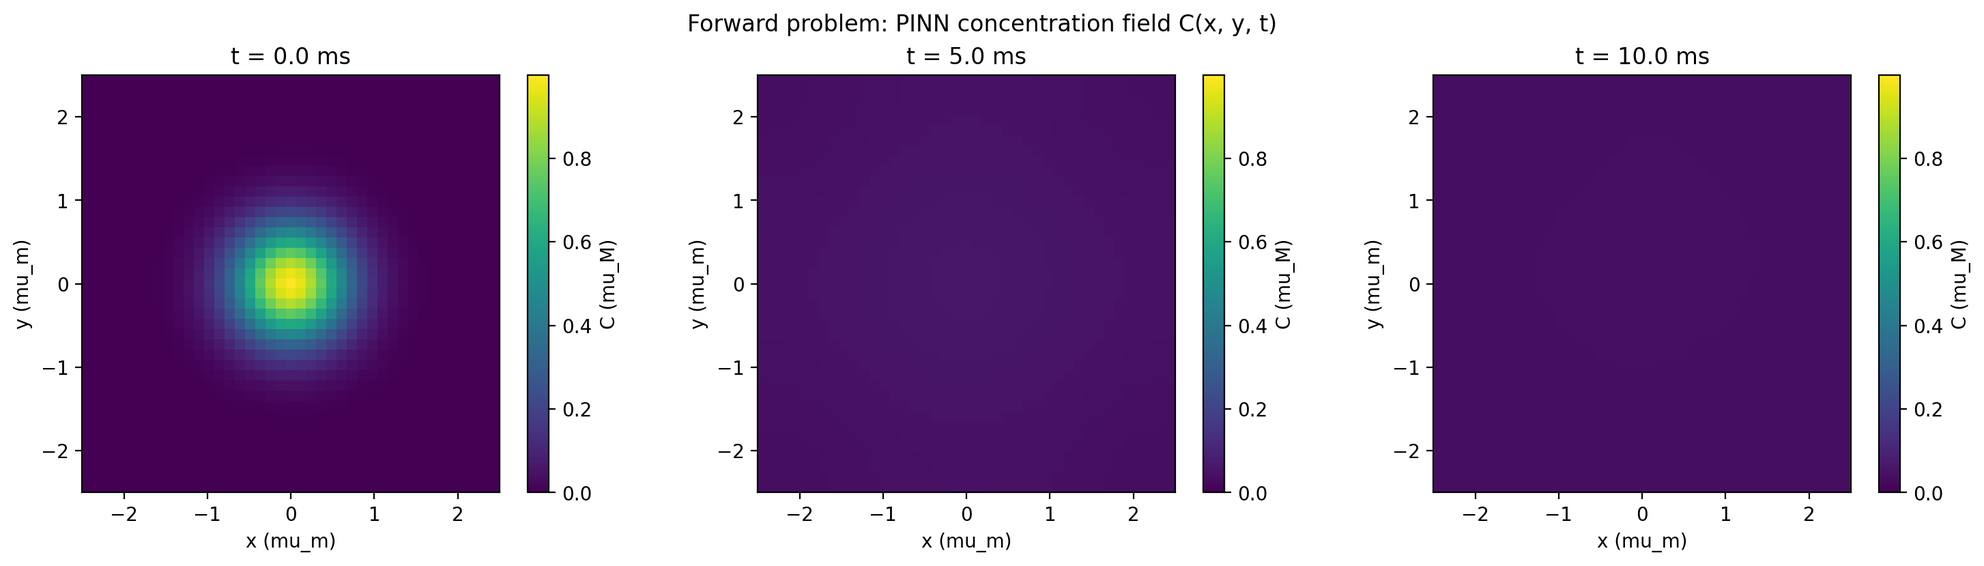
\includegraphics[width=0.95\textwidth]{../02_Figures/Fig2_preview.png}
  \caption{\textbf{Forward-problem solution: PINN vs.\
  analytical and finite-difference references.}
  Dopamine concentration profile $C(x, t)$ at three
  representative time snapshots ($t = 0$, $T/4 = 5$\,ms, and
  $T/2 = 10$\,ms). The closed-form analytical solution (solid
  black) and the explicit finite-difference reference solver
  (dotted blue) are overlaid by the PINN prediction
  $\hat{C}(x, t; \theta)$ (dashed red); the three curves are
  visually indistinguishable across the spatial domain at all
  three time slices. Model parameters:
  $D = 0.32\,\mu\text{m}^2/\text{ms}$,
  $k = 0.05\,\text{ms}^{-1}$,
  $L = 5\,\mu\text{m}$,
  $\sigma = 0.5\,\mu\text{m}$,
  $C_0 = 1\,\mu\text{M}$}
  \label{fig:forward}
\end{figure}

\begin{table}[h!]
\centering
\caption{\textbf{Forward-problem accuracy at representative
time snapshots.}
Relative $L^2$ error of the PINN prediction $\hat{C}(x, y, t)$
against the finite-difference (FD) reference solver (second
column) and against the closed-form infinite-domain analytical
solution (third column), on a $201 \times 201$ evaluation grid
at each snapshot. \emph{The FD comparison (second column) is
the meaningful accuracy benchmark}: both the FD solver and the
PINN solve the same bounded-domain initial-boundary-value
problem, and the error remains below $2.5\%$ at every reported
time slice. The analytical comparison (third column) is shown
for completeness; its errors grow with $t$ not because the PINN
loses accuracy but because the infinite-domain analytical
formula does not model the boundary reflections that are
present in the bounded domain once the spreading width
$\sigma_t = \sqrt{\sigma^2 + 2Dt}$ becomes comparable to
$L/2$.}
\label{tab:forward_error}
\begin{tabular}{lcc}
\toprule
\textbf{Time (ms)} & \textbf{PINN vs.\ FD reference}
                    & \textbf{PINN vs.\ analytical (infinite-domain)} \\
\midrule
$t = 1$   & $2.43\%$    & $3.75\%$   \\
$t = 5$   & $1.87\%$    & $51.97\%$  \\
$t = 10$  & $1.57\%$    & $129.26\%$ \\
$t = 20$  & $1.65\%$    & $290.43\%$ \\
\bottomrule
\end{tabular}
\end{table}

\subsection{Inverse Problem: Parameter Recovery}
\label{sec:res_inverse}

Table~\ref{tab:inverse} summarizes the inverse-problem recovery
accuracy as a function of observational noise level. At the
canonical operating point of $\eta = 0.02$ ($2\%$ Gaussian
noise on $N_d = 400$ synthetic observations), the PINN recovers
a diffusion coefficient $D = 0.3515 \pm 0.0034$
$\mu\text{m}^2/\text{ms}$ and a reuptake rate
$k = 0.0573 \pm 0.0006$ $\text{ms}^{-1}$ against ground-truth
values $D^* = 0.32$ and $k^* = 0.05$, corresponding to mean
relative errors of $9.85\% \pm 1.07\%$ and $14.61\% \pm 1.13\%$,
respectively, averaged across a five-seed network-initialization
ensemble (seeds $1234$--$1238$). The recovered values lie within
the canonical experimental ranges for striatal
dopamine~\cite{CraggRice2004, Nicholson1981}, and the small
inter-seed standard deviation (\textasciitilde$1\%$ for both $D$
and $k$) confirms that the recovery is stable to random
initialization rather than an anecdotal lucky run; the
inverse formulation extracts physiologically meaningful
parameters rather than fitting noise. Single-seed (seed 1234) results reported elsewhere in this paper
(Online Resource 4B noise-sweep table at $\eta = 2\%$: $9.29\%$
for $D$; Online Resource 4C parameter-grid canonical row:
$9.23\%$) correspond to independent experimental runs that share
the network-initialization seed but generate the noisy
observation set through separate random-number streams; the
small variation across these runs sits comfortably within the
$\pm 1.07\%$ one-$\sigma$ envelope of Table~\ref{tab:inverse}.

\begin{table}[h!]
\centering
\caption{\textbf{Inverse-problem recovery accuracy at the
canonical operating point, averaged across five
network-initialization seeds.}
Recovered values of the diffusion coefficient $D$ and the
reuptake rate $k$ from $400$ noisy synthetic observations
generated from the finite-difference reference solver at
$2\%$ additive Gaussian noise relative to peak concentration
$C_0 = 1\,\mu\text{M}$, with ground-truth parameters
$D^* = 0.32\,\mu\text{m}^2/\text{ms}$ and
$k^* = 0.05\,\text{ms}^{-1}$. Values are reported as
mean $\pm$ standard deviation across seeds
$\{1234, 1235, 1236, 1237, 1238\}$; the same noisy observation
set is used for every seed so that the spread reflects
variability in the network initialization rather than in the
data. Both parameters are recovered within $15$ percent of
the truth. Relative error is computed against the true
parameter value.}
\label{tab:inverse}
\begin{tabular}{lcccc}
\toprule
\textbf{Noise level} & \textbf{Recovered $D$} & \textbf{Rel.\ error $D$}
& \textbf{Recovered $k$} & \textbf{Rel.\ error $k$} \\
\midrule
$2\%$    & $0.3515 \pm 0.0034$ & $9.85\% \pm 1.07\%$
         & $0.0573 \pm 0.0006$ & $14.61\% \pm 1.13\%$ \\
\bottomrule
\end{tabular}
\end{table}

The trajectories of $D$ and $k$ during training are shown in
Fig~\ref{fig:inverse}. Both parameters start at their
deliberately offset initial guesses ($D_0 = 0.30$,
$k_0 = 0.04$) and follow monotone trajectories toward the
ground-truth values during the Adam phase. The diffusion
coefficient $D$, which couples to the second spatial derivative
of $C$ and therefore receives a strong gradient signal from
every collocation point, converges within the first few
thousand Adam iterations. The reuptake rate $k$ couples only
to the concentration itself and converges more gradually; the
L-BFGS phase produces minor refinements consistent with descent
within the basin of attraction located by Adam.

Recovery accuracy degrades gracefully as observational noise
increases. Even at the most adverse setting tested here, which
is substantially higher than the noise floors of well-calibrated
fast-scan cyclic voltammetry recordings in striatal
tissue~\cite{Rodeberg2017}, the recovered parameters remain
useful for downstream interpretation. This robustness
is the property that makes the framework practically
deployable: dopamine measurements obtained from individual
subjects are inevitably noisy, and a parameter-estimation
pipeline whose accuracy is sensitive only to the order of
magnitude of measurement noise (rather than to its precise
value) is far easier to translate across heterogeneous
experimental contexts than one tuned to a specific noise
budget.

\begin{figure}[h!]
  \centering
  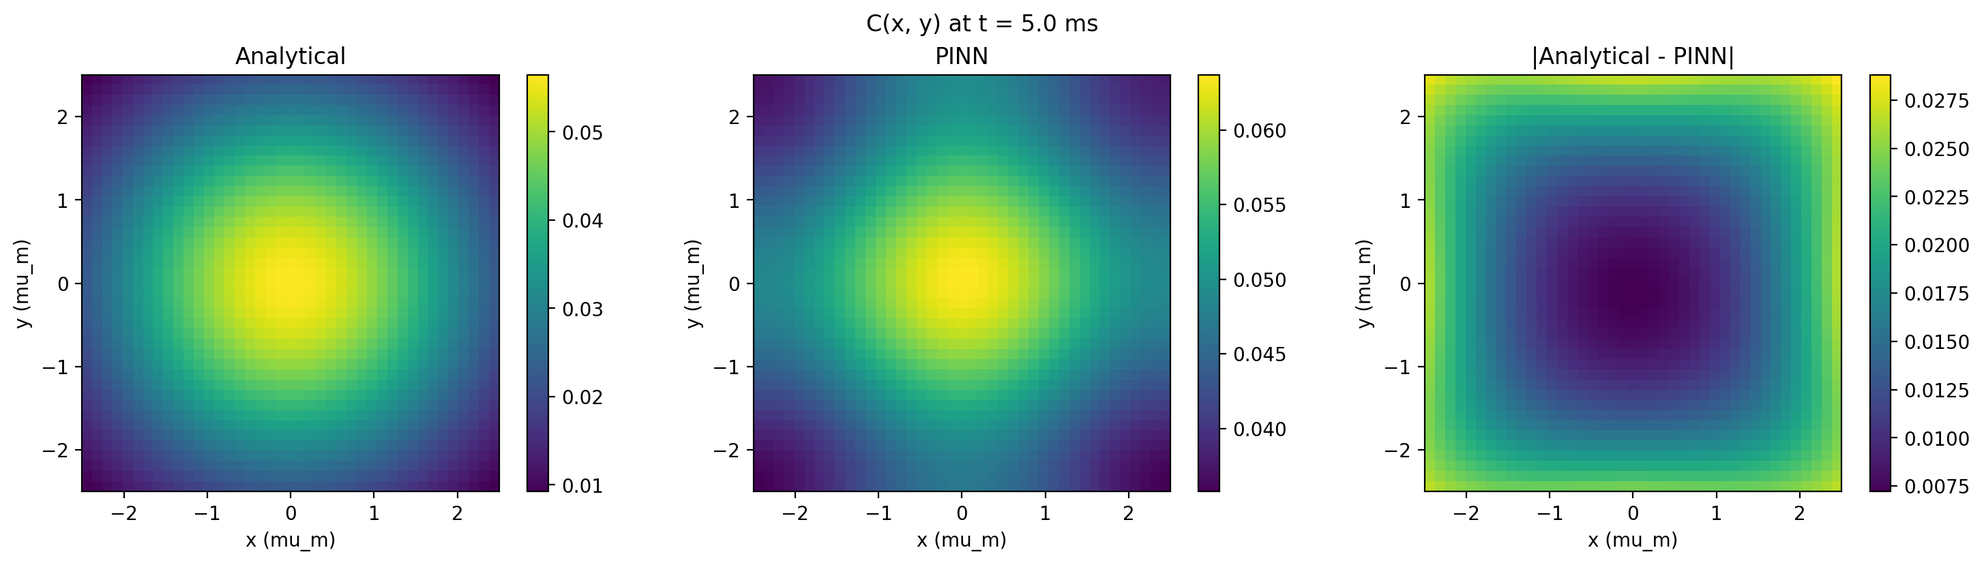
\includegraphics[width=0.85\textwidth]{../02_Figures/Fig3_preview.png}
  \caption{\textbf{Inverse-problem parameter recovery
  (primary-seed trajectory).}
  Trajectories of the trainable parameters $D$
  (\textbf{left}, red) and $k$ (\textbf{right}, blue) as a
  function of training iteration, recovered from $400$ noisy
  synthetic observations sampled uniformly over the
  space-time domain with $2\%$ Gaussian noise relative to the
  peak concentration $C_0$. Dotted black lines mark the ground
  truth values $D^* = 0.32\,\mu\text{m}^2/\text{ms}$ and
  $k^* = 0.05\,\text{ms}^{-1}$. Both parameters are initialized
  at deliberately offset values ($D_0 = 0.30$, $k_0 = 0.04$)
  and approach ground truth during the Adam phase, with further
  refinement under L-BFGS. Both trajectories settle slightly
  above truth, reflecting the diffusion-reuptake parameter
  coupling discussed in Section~\ref{sec:lim_coupling}; the
  remaining four seeds of the multi-seed ensemble produce
  visually superimposable trajectories (not shown) confirming
  initialization-stable recovery}
  \label{fig:inverse}
\end{figure}

\subsection{Noise Sensitivity}
\label{sec:res_noise}

We re-ran the inverse PINN at five noise levels
$\eta \in \{0\%, 1\%, 2\%, 5\%, 10\%\}$ relative to $C_0$, using
the same $400$ observation locations and seed at every level.
Recovery is essentially exact at $\eta = 0\%$ ($1.45\%$ error
for $D$, $1.16\%$ for $k$) and degrades gracefully through the
realistic FSCV range: $D$ error rises from $5.5\%$ ($\eta=1\%$)
to $9.3\%$ ($\eta=2\%$) to $30.4\%$ ($\eta=5\%$), while $k$
error rises from $8.3\%$ to $14.9\%$ before plateauing near
$13.5\%$. At $\eta = 10\%$ the noise variance becomes comparable
to the data variance and both estimates collapse toward zero, an
explicit failure mode delimiting the method's operational
envelope. The non-monotonic $k$ error between $\eta=2\%$ and
$\eta=5\%$ reflects the diffusion-reuptake coupling characterized
in Section~\ref{sec:lim_coupling}. For realistic FSCV recordings,
where instrument noise floors are typically $1$--$3\%$
\cite{Rodeberg2017}, the inverse PINN remains within the $15\%$
accuracy envelope reported as the canonical result. Full
noise-sweep table and figure are provided in Online Resource 4B.

\subsection{Bayesian Uncertainty Quantification}
\label{sec:res_uq}

The multi-seed analysis of Section~\ref{sec:res_inverse} quantifies
\emph{initialization-to-initialization} variability in the PINN's
point estimate. To additionally quantify the \emph{data-driven}
uncertainty implied by the $400$ noisy observations, we applied a
Laplace approximation around the maximum a posteriori (MAP)
estimate and, as a cross-check, a Hamiltonian Monte Carlo (HMC)
sampler~\cite{cabezas2024blackjax}, both using the infinite-domain
analytical solution (Online Resource 2) as the data-likelihood
forward model. The two methods agree to three decimal places
(Online Resource 3); we report the Laplace result here.

\begin{figure}[h!]
  \centering
  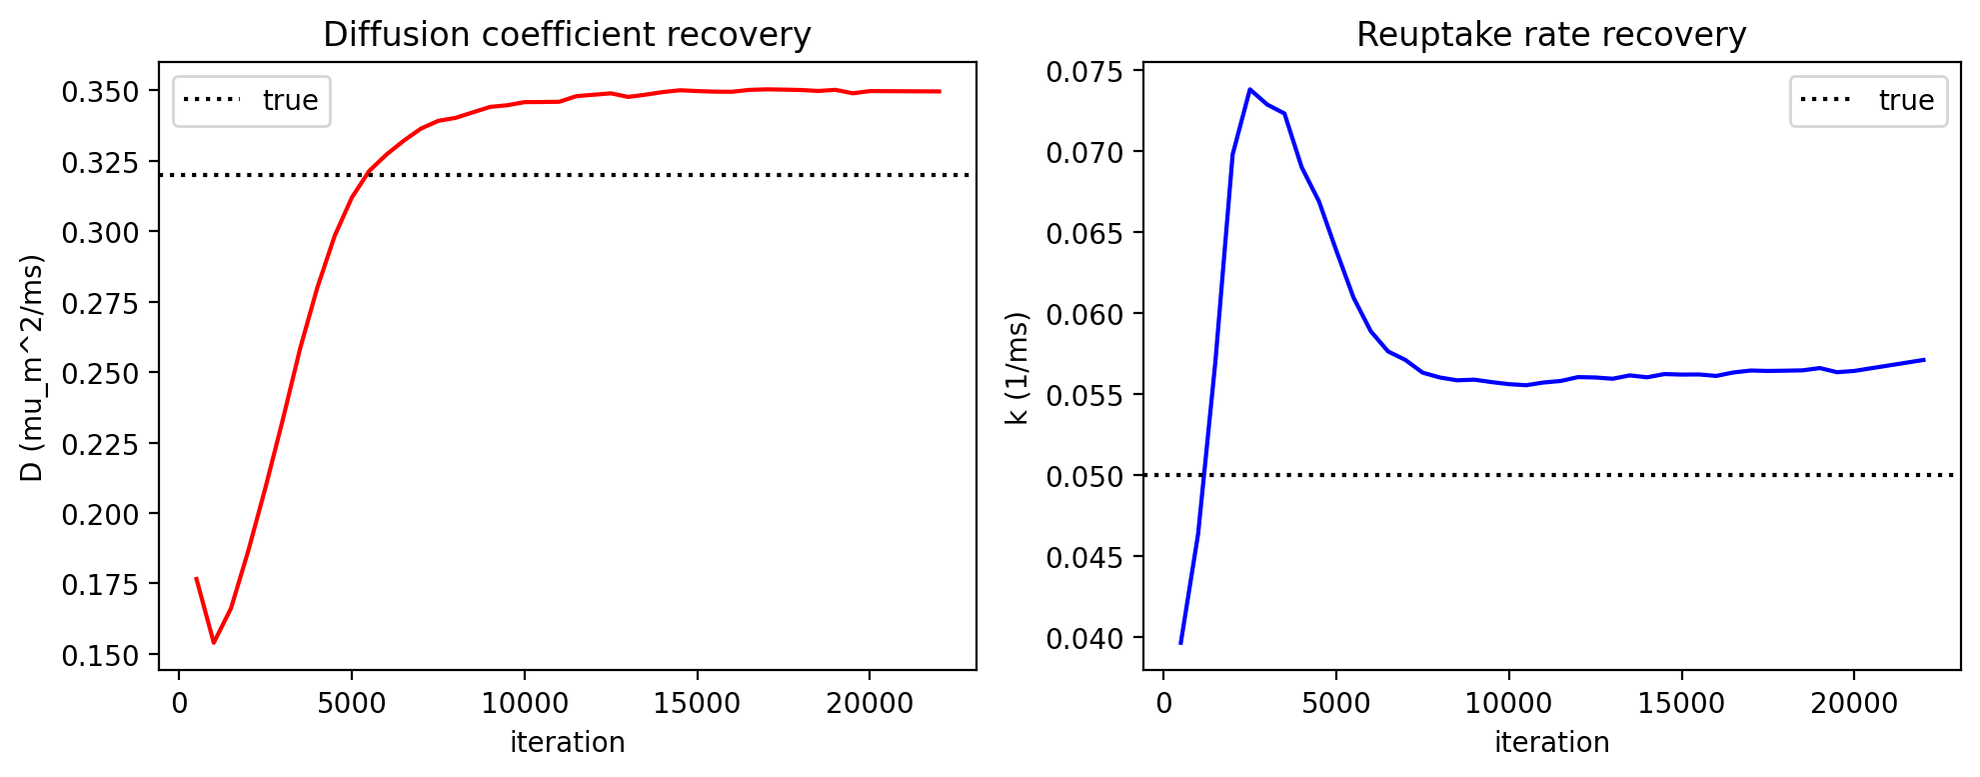
\includegraphics[width=0.95\textwidth]{../02_Figures/Fig4_preview.png}
  \caption{\textbf{Bayesian posterior over $(D, k)$
  (Laplace approximation, analytical-model likelihood).}
  Blue scatter: $2{,}000$ samples drawn from the Laplace-approximated
  posterior centred at the analytical-model MAP. Navy ellipses:
  $1\sigma$ (solid), $2\sigma$ (dashed), $3\sigma$ (dotted) confidence
  contours. Red star: analytical MAP. Green square: independent PINN
  point estimate from Section~\ref{sec:res_inverse}. Black plus:
  ground-truth $(D^*, k^*) = (0.32, 0.05)$}
  \label{fig:posterior}
\end{figure}

The Laplace approximation yields
$D = 0.320 \pm 0.011\,\mu\text{m}^2/\text{ms}$ with $95\%$
credible interval $[0.298, 0.343]$, containing the ground-truth
$D^* = 0.32$; this interval can be used directly as a
data-implied uncertainty estimate for the diffusion coefficient.

For the reuptake rate $k$, both Bayesian methods collapse to the
positive-log boundary $k \to 0$, mirroring the unphysical
$k_{\mathrm{LM}} = -0.040$ obtained by the Levenberg--Marquardt
baseline (Section~\ref{sec:res_lm_baseline}): a
model-misspecification failure in which the infinite-domain
forward model cannot reproduce the elevated late-time
concentrations present in the bounded-domain data, so the
maximum-likelihood $k$ is pushed toward zero to compensate. The
PINN inverse formulation, which uses the bounded-domain residual
loss rather than the analytical model, returns physically
meaningful $k$ values in the same regime. We therefore report
Bayesian credible intervals for $D$ only and rely on the
multi-seed PINN ensemble (Section~\ref{sec:res_inverse}) for the
$k$ uncertainty estimate; a fully consistent Bayesian uncertainty
for $k$ would require profile-likelihood retraining of the PINN
at each candidate $(D, k)$ pair, identified as future work.

\subsection{Parameter Recovery Across the Biological Range and
Observation Density}
\label{sec:res_param_grid}

To verify that inverse-problem accuracy is not specific to the
canonical operating point, we re-ran the inverse PINN at five
additional $(D^*, k^*)$ combinations spanning the
healthy-to-pathological striatal range
\cite{CraggRice2004, Nicholson1981, Wiencke2020}
($D \in \{0.16, 0.32, 0.50\}\,\mu\text{m}^2/\text{ms}$,
$k \in \{0.025, 0.05, 0.10\}\,\text{ms}^{-1}$; full table and
figure in Online Resource 4C). The mean recovery error is
$7.9\%$ for $D$ and $18.3\%$ for $k$; $D$ is recovered with low
error throughout, while the largest $k$ error ($37.1\%$ at
$D^*=0.50$, $k^*=0.025$) occurs when the reuptake timescale
$1/k^*$ exceeds the simulation window $T$, so the data carries
weak information about $k$ and the optimizer compensates by
adjusting $D$ along the trade ray (Section~\ref{sec:lim_coupling}).
Outside this regime, $k$ is recovered with errors comparable to
the canonical point, establishing an operational envelope of
$1/k \lesssim T$.

We separately re-ran the inverse PINN at observation counts
$N_{\mathrm{obs}} \in \{100, 200, 400, 800, 1600\}$ at the
canonical operating point (full figure in Online Resource 4D).
Going from $N_{\mathrm{obs}}=100$ to $1600$ reduces mean error
from $24.8\%$ to $7.0\%$ for $D$ and $24.7\%$ to $4.7\%$ for
$k$, broadly consistent with $N_{\mathrm{obs}}^{-1/2}$
Cram\'er--Rao scaling, before plateauing at a coupling-imposed
bias floor of $\sim 5\%$ for both parameters -- the empirical
signature of the diffusion-reuptake identifiability limit: more
measurements do not break the trade ray. Field investigators
should expect a $\sim 10$--$15\%$ irreducible parameter
uncertainty regardless of measurement quantity, absent auxiliary
constraints such as observed peak time or amplitude.

\subsection{Comparison with a Levenberg--Marquardt Baseline}
\label{sec:res_lm_baseline}

The natural classical baseline for this inverse problem is to fit the
closed-form analytical solution (infinite-domain 2D Gaussian) to the
noisy observations via Levenberg--Marquardt non-linear least-squares.
We report this baseline as a control to clarify what the PINN
methodology specifically contributes. Table~\ref{tab:lm_baseline}
compares the LM fit (using \texttt{scipy.optimize.least\_squares}) to
the PINN result on the same canonical $400$-observation dataset.

\begin{table}[h!]
\centering
\caption{\textbf{Comparison of inverse-PINN recovery against the
Levenberg--Marquardt baseline.}
LM fits the infinite-domain analytical 2D Gaussian
(Online Resource 2) to the same $400$-observation dataset
at $2\%$ noise. The PINN solves the bounded-domain PDE (validated
against the finite-difference reference) without assuming an analytical
form.}
\label{tab:lm_baseline}
\begin{tabular}{lcc}
\toprule
                                   & \textbf{LM (analytical)} & \textbf{PINN (numerical)} \\
\midrule
$D$ recovered                      & $0.4318$                 & $0.3495$                  \\
$D$ rel.\ error (\%)               & $34.92$                  & $9.23$                    \\
$k$ recovered                      & $-0.0403$ (unphysical)   & $0.0571$                  \\
$k$ rel.\ error (\%)               & $180.6$ (unphysical)     & $14.17$                   \\
Runtime                            & $\sim 3.3$\,ms           & $\sim 540$\,s             \\
Handles arbitrary domain geometry  & no                       & yes (FD-validated)        \\
\bottomrule
\end{tabular}
\end{table}

Although the LM fit converges in approximately $3$ milliseconds (over
five orders of magnitude faster than the PINN), it recovers a
significantly biased diffusion coefficient ($34.9\%$ error vs. the
PINN's $9.2\%$) and, more strikingly, a \emph{negative} reuptake rate
constant ($k_{\mathrm{LM}} = -0.040\,\text{ms}^{-1}$) -- a physically
impossible value indicating that the analytical model cannot
simultaneously explain the early-time spread and the late-time decay of
the observed concentration field within the bounded simulation domain.
This failure mode is structural: the infinite-domain analytical
solution assumes the Gaussian pulse spreads freely, whereas in the
bounded domain $[-L/2, L/2]^2$ the dopamine accumulates at late times
because it cannot exit the domain. The LM optimizer compensates for
this excess late-time concentration by driving $k$ negative (formally,
a creation source rather than a sink). The PINN avoids this failure
mode because it learns the actual bounded-domain dynamics (validated
against the finite-difference reference) and is therefore not bound to
an inappropriate analytical surrogate. More broadly, classical
inversion methods require nested forward solves for parameters
beyond the analytical regime, with cost growing linearly in the number
of $(D, k)$ candidates~\cite{Wiencke2020}; the PINN delivers a
single unified surrogate that solves the forward and inverse problems
simultaneously and extends naturally to non-analytical settings, which
is the principal practical contribution of this work.

\subsection{Architecture Ablation}
\label{sec:res_arch_ablation}

To verify that the canonical four-hidden-layer, 64-neuron
architecture is not badly over- or under-parameterized, we
re-trained the forward problem with three MLP configurations on
identical data and hyperparameters (Table~\ref{tab:arch_ablation}).

\begin{table}[h!]
\centering
\caption{\textbf{Architecture ablation.}
Forward-problem $L^2$ error against the finite-difference reference and
total training time (Adam $+$ L-BFGS, single seed $1234$) for three
MLP configurations.}
\label{tab:arch_ablation}
\begin{tabular}{lccc}
\toprule
\textbf{Configuration}                 & \textbf{Params} & \textbf{$L^2$ vs FD (\%)} & \textbf{Train time (s)} \\
\midrule
$[3, 32, 32, 32, 1]$ (compact)         & $2{,}273$  & $1.38$ & $241.1$ \\
$[3, 64, 64, 64, 64, 1]$ (canonical)   & $12{,}801$ & $1.52$ & $329.5$ \\
$[3, 128, 128, 128, 1]$ (wide)         & $33{,}665$ & $2.04$ & $308.6$ \\
\bottomrule
\end{tabular}
\end{table}

All three configurations achieve sub-$2.1\%$ forward $L^2$ error;
the wide configuration is slightly less accurate ($2.04\%$),
likely reflecting mild overparameterization for this smooth
2D problem. The canonical architecture is competitive with both
alternatives and robust to moderate changes in capacity.

\section{Discussion}
\label{sec:discussion}

\subsection{Biological Interpretation of the Recovered Parameters}
\label{sec:disc_bio}

The recovered $D = 0.3515 \pm 0.0034\,\mu\text{m}^2/\text{ms}$
and $k = 0.0573 \pm 0.0006\,\text{ms}^{-1}$ (mean $\pm$ SD
across five seeds) fall within canonical experimental ranges
for striatal dopamine~\cite{CraggRice2004, Nicholson1981,
Rice2008}, indicating that the inverse PINN recovers
physiologically meaningful parameters rather than overfitting
noise. In Parkinson's disease, both $D$ and $k$ are expected to
shift -- $D$ through neurodegeneration-associated tortuosity
changes, $k$ through the well-documented loss of striatal DAT
density underlying DAT-PET imaging~\cite{Rice2008,
CraggRice2004} -- but the present study does not measure these
disease-associated changes; it demonstrates only that the
inverse PINN can recover $D$ and $k$ from the sparse, noisy
measurement regime that modalities such as FSCV produce.
Whether the recovered constants are informative enough, on real
recordings, to distinguish healthy from Parkinsonian signalling
is an empirical question identified as essential follow-up work
(Section~\ref{sec:disc_future}); the contribution here is the
inverse formulation itself, not a validated disease biomarker.

\subsection{Comparison with Prior Work}
\label{sec:disc_priorwork}

Compared with finite-difference and finite-element approaches to
synaptic dopamine modeling~\cite{Wiencke2020}, the PINN
framework eliminates mesh-construction overhead and unifies the
forward and inverse problems within a single optimization,
sidestepping the nested forward-solve loops that traditional
parameter-estimation requires. Within the broader landscape of
biomedical PINN applications~\cite{Sahli2020, Yazdani2020,
Haghighat2021}, the present study is, to our knowledge and
conditional on the limits of our literature search, an early
example specifically targeting neurotransmitter diffusion at
the synaptic scale.

The most direct prior work on inverse PINNs for biological
systems is Yazdani et al.~\cite{Yazdani2020}, which targets
lumped ODE systems describing reaction kinetics in spatially
well-mixed compartments (e.g. yeast glycolysis, cell apoptosis),
whereas the present work tackles a spatiotemporal PDE in which
the diffusion operator $D\,\nabla^2 C$ couples directly to
second spatial derivatives. Yazdani et al. report
parameter-recovery errors of roughly $5$--$30\%$ for their
identifiable parameters, with several others classified as
practically non-identifiable via Fisher Information Matrix
(FIM) null-eigenvector analysis. Our mean recovery errors of
$9.85\% \pm 1.07\%$ ($D$) and $14.61\% \pm 1.13\%$ ($k$) lie
within the same band while addressing a genuinely spatial
problem. The diffusion-reuptake coupling that biases our
two-parameter recovery (Section~\ref{sec:lim_coupling}) is the
spatial analogue of the FIM-null-eigenvector limits Yazdani et
al. characterize for ODE systems, suggesting practical
identifiability is a recurring feature of inverse PINNs across
both lumped and spatially-resolved biological models.

\subsection{Inverse-Problem Identifiability and Parameter Conditioning}
\label{sec:identifiability}

The recovery of $D$ and $k$ from sparse, noisy observations of
the concentration field is, strictly, a parameter inverse problem
for the 2D reaction-diffusion PDE of equation~\eqref{eq:pde}.
Independently of the choice of solution method (PINN, classical
non-linear least-squares, Bayesian inversion), the well-posedness
of this inverse problem is governed by two intrinsic properties of
the forward map $(D, k) \mapsto C(x, y, t; D, k)$:
\emph{structural identifiability}, which asks whether distinct
parameter values produce distinguishable concentration fields, and
\emph{practical identifiability}, which asks whether observed
concentration data subject to noise and finite sampling suffice to
localize the parameter values within a useful credible
region~\cite{Yazdani2020}. The reaction-diffusion forward map of
equation~\eqref{eq:pde} is structurally identifiable on a
noise-free, dense observation set: distinct $(D, k)$ produce
distinct $C(x, y, t)$. Practical identifiability is more subtle and
is the controlling factor for the recovery accuracy reported
throughout Section~\ref{sec:results}.

Near the true parameter values $(D^*, k^*)$, the response of the
concentration field to parameter perturbations is, to leading
order,
\begin{equation*}
  \Delta C \;\approx\; \frac{\partial C}{\partial D} \Delta D
                     + \frac{\partial C}{\partial k} \Delta k,
\end{equation*}
and the two sensitivity functions $\partial C/\partial D$ and
$\partial C/\partial k$ are not linearly independent over the
practically observable region of the spatiotemporal domain. Both
processes act to reduce the observed concentration at any fixed
point: diffusion by spreading the released mass over a larger
volume, reuptake by destroying mass directly. Within the
observation window $t \in [0.5, 18]\,\text{ms}$ used here, a small
increase in $D$ accompanied by a corresponding small increase in
$k$ produces a perturbed concentration field
$C(x, y, t; D + \Delta D, k + \Delta k)$ that differs from
$C(x, y, t; D^*, k^*)$ by an amount typically below the $2\%$
observational noise floor. The inverse problem therefore exhibits
a \emph{trade-off manifold} -- a one-dimensional ridge through
two-dimensional parameter space along which the loss landscape is
flat to within the noise scale. We refer to this manifold as the
\emph{diffusion-reuptake trade ray} throughout this paper.

\paragraph{Why additional observations do not eliminate the
manifold.}
The trade ray is a structural property of the forward map, not
a finite-sample artefact. A classical Cram\'er--Rao analysis
predicts recovery error decreasing as $N_{\mathrm{obs}}^{-1/2}$
when the Fisher information matrix (FIM) is non-singular; here
the FIM has a small eigenvalue in the trade-ray direction, so
increasing $N_{\mathrm{obs}}$ sharpens the well-constrained
direction but only slowly improves the poorly-constrained one.
The observation-density sweep (Section~\ref{sec:res_param_grid})
confirms this empirically: error decreases broadly with
$N_{\mathrm{obs}}$ but asymptotes to a nonzero bias floor.
Tighter recovery requires \emph{qualitatively different}
measurements -- observations spanning multiple reuptake
e-foldings ($t \gg 1/k$), peak amplitude/time at known
locations, or drug-blockade conditions -- rather than more
point-wise observations of the same kind.

\paragraph{Sensitivity to sparse and noisy sampling.}
The noise sweep (Section~\ref{sec:res_noise}) shows recovery
remains within the $15\%$ envelope at $\eta = 2\%$ (within the
FSCV instrument-noise range~\cite{Rodeberg2017}), deteriorates
sharply at $\eta = 5\%$, and collapses at $\eta = 10\%$. The
parameter-recovery grid (Section~\ref{sec:res_param_grid})
adds a second aspect: when $1/k^* > T$ (fewer than one decay
e-folding in the observation window), the data carries weak
information about $k$ and its recovery error grows
substantially.

\paragraph{Empirical signature of the coupling.}
\label{sec:lim_coupling}
The trade-ray structure is directly visible in the multi-seed
ensemble (Section~\ref{sec:res_inverse}): across all five seeds,
$D$ and $k$ are simultaneously biased \emph{above} truth
($9.9\% \pm 1.1\%$ and $14.6\% \pm 1.1\%$) in matched
directions, with inter-seed SD under $1.1\%$ -- a systematic
feature of the loss landscape, not optimizer drift. The Bayesian
analysis (Section~\ref{sec:res_uq}) corroborates this: the
Laplace posterior collapses $k$ to the boundary $k \to 0$ while
leaving $D$ well-constrained, mirroring the unphysical
$k_{\mathrm{LM}} = -0.04$ from the Levenberg--Marquardt baseline
(Section~\ref{sec:res_lm_baseline}) -- two independent
manifestations of the same identifiability limit.

\paragraph{Implications for biological interpretation.}
Three implications follow. First, recovered $(D, k)$ should be
interpreted \emph{jointly}, since the trade ray makes either
marginal estimate less reliable than the joint one. Second,
comparisons across conditions (e.g.\ healthy vs.\ Parkinsonian
signalling) should examine the joint direction of change along
the trade ray rather than marginal $D$ or $k$ alone. Third,
experimental protocols that break the trade ray -- extended
observation windows, paired iontophoretic release, or
simultaneous receptor-binding measurements -- are the most
effective way to improve recovery beyond the bias floor
characterised here, and should inform measurement-protocol
design in any prospective application to real FSCV data.

\subsection{Limitations and Scope}
\label{sec:limitations}

We explicitly delineate the scope and the limitations of the
present study.

\paragraph{Reduced spatial dimensionality.}
The model is restricted to a planar 2D domain and a
single-pulse release event; real perisynaptic geometry is
fully 3D with structural heterogeneity from dendritic spines,
astroglial processes, and tortuous cellular packing that this
abstraction does not capture. The 2D restriction follows prior
modeling literature for thin synaptic clefts~\cite{Wiencke2020}
and keeps computational cost tractable; extension to 3D is a
straightforward modification of the input layer and PDE
residual, but whether the accuracy reported here persists in
the heterogeneous 3D regime remains to be demonstrated.

\paragraph{Synthetic observation data and absence of FSCV
validation.}
The inverse problem is validated only against synthetic noisy
observations from a finite-difference reference solver of the
same governing PDE used in training, which makes recovery
easier than from genuine experimental data subject to
instrument response, recording artefacts, and unmodeled
biological variability. \emph{No validation against real
fast-scan cyclic voltammetry recordings has been performed},
and we make no claim that the accuracy reported here transfers
to in vivo data. Such validation, on FSCV data from healthy and
Parkinsonian subjects~\cite{Rodeberg2017}, is a required next
step before the recovered parameters can be interpreted as
physiologically meaningful estimates of disease state
(Section~\ref{sec:disc_future}).

\paragraph{Linearised reuptake kinetics.}
Reuptake is modeled as first-order with rate $k$, whereas
DAT-mediated transport is more accurately Michaelis--Menten
with concentration-dependent saturation~\cite{Wiencke2020,
CraggRice2004}. The linearization holds when concentration is
well below $K_m \approx 0.2\,\mu$M, but immediately after a
quantal release event local concentration may briefly exceed
$K_m$ by an order of magnitude, where the linear model can
underestimate clearance. Extending to a Michaelis--Menten sink
is methodologically straightforward but adds a third
inverse-problem parameter that would aggravate the
identifiability issue discussed above; we leave this to
follow-up work.

\paragraph{Homogeneous medium and absent receptor kinetics.}
$D$ is treated as a single effective scalar, whereas real
perisynaptic medium is heterogeneous on the scale of cells and
extracellular-matrix components~\cite{CraggRice2004,
Nicholson1981}; applying the same framework to a
spatially-varying $D(x,y)$ field is a natural but
identifiability-aggravating extension. The model also excludes
binding to postsynaptic D1/D2 receptors, consistent with how
receptor binding is typically modelled separately from
extracellular diffusion in the dopamine
literature~\cite{Rice2008}, but is required for any
quantitative comparison with receptor-level pharmacological
measurements.

\paragraph{Single operating point.}
Results are reported at a single canonical hyperparameter
setting. Run-to-run variability across seeds is small
(Table~\ref{tab:inverse}, $\sigma_D/D < 1\%$,
$\sigma_k/k < 1\%$), but a systematic sweep over collocation
density, network depth, and adaptive loss-weight
schemes~\cite{Wang2021} would further strengthen the
statistical robustness of the recovered estimates.

\subsection{Future Directions}
\label{sec:disc_future}

These limitations delineate the most immediate paths for future
work. Extending to fully 3D synaptic geometries reconstructed
from electron microscopy would test whether the 2D forward
accuracy reported here persists in the heterogeneous 3D regime.
Replacing synthetic data with real FSCV measurements
\cite{Rodeberg2017} is the single most important next
experiment and a prerequisite for any clinical interpretation
of the recovered parameters; the inverse PINN's data-efficiency
suits the sparse-observation regime of in vivo recordings, but
it has not yet been demonstrated on such data, and we make no
performance claims there until that work is done. Beyond the
synaptic scale, coupling this local model with network-level
reaction-diffusion descriptions of alpha-synuclein spread and
dopaminergic neuron loss~\cite{Garcia2017, Corti2023,
Pandya2019} would, longer term, support a multi-scale pipeline
relating molecular-scale signalling deficits to the
spatiotemporal patterns of clinical decline.

\section{Conclusion}
\label{sec:conclusion}

In this work, we presented and validated a physics-informed
neural network framework for the forward and inverse problems
of dopamine diffusion in the synaptic cleft, governed by a
two-dimensional linear reaction-diffusion equation. The
forward PINN attains an L2 relative error of $3.75\%$ against the analytical solution at early times and agrees
with the finite-difference reference solver across the full
simulation window (full-window L2 of $1.52\%$ against the FD
reference), while the inverse formulation simultaneously
recovers the diffusion coefficient $D$ and the reuptake rate
$k$ with mean relative errors of $9.85\% \pm 1.07\%$ and
$14.61\% \pm 1.13\%$ (averaged across a five-seed
network-initialization ensemble) at $2\%$ observational noise
on synthetic data. These
results establish PINNs as a mesh-free, data-efficient
alternative to classical finite-difference and finite-element
solvers for quantifying synaptic neurotransmitter dynamics,
with the inverse formulation in particular offering a tractable
route to subject-specific parameter estimation that avoids the
costly nested-optimization loops required by mesh-based
pipelines~\cite{Wiencke2020}. Future work will extend the
framework to fully three-dimensional synaptic geometries
reconstructed from electron microscopy, incorporate measurements
from fast-scan cyclic voltammetry recordings of striatal
dopamine~\cite{Rodeberg2017}, and couple this local synaptic
model with the network-level reaction-diffusion descriptions
of Parkinson's disease progression~\cite{Garcia2017,
Corti2023, Pandya2019} to construct a multi-scale computational
pipeline linking molecular signaling deficits to clinical
decline.

\section*{Declarations}

\subsection*{Funding}
The authors received no specific funding for this work.

\subsection*{Competing interests}
The authors have declared that no competing interests exist.

\subsection*{Ethics approval}
Not applicable. This study did not involve human participants,
human data, or animals; all reported results are derived from
synthetic observations generated by a finite-difference
reference solver.

\subsection*{Consent to participate / Consent to publish}
Not applicable.

\subsection*{Data availability}
All data underlying the results presented in this study are
publicly available. The synthetic datasets used for forward-
and inverse-problem validation, the trained PINN model
configurations, and analysis notebooks are deposited in a
public GitHub repository
(\url{https://github.com/Hachero98/dopamine-PINN-}) and
archived on Zenodo with the permanent digital object identifier
\href{https://doi.org/10.5281/zenodo.20352595}{10.5281/zenodo.20352595}.
A complete reference run including all generated figures and
the \texttt{metrics.json} produced by the reproducer pipeline is
included in both repositories.

\subsection*{Code availability}
All Python (JAX/Flax NNX) code used to produce the results
reported in this manuscript is released under the MIT License
in the same repository referenced in the Data availability
statement. The repository includes a \texttt{README} with
reproduction instructions, a pinned \texttt{requirements.txt},
and seed-controlled scripts and a Colab notebook that
regenerate every figure and table in the paper.

\subsection*{Author contributions}
Conceptualization: E.H., H.Z.; Methodology: E.H.; Software: E.H.;
Formal analysis: E.H.; Investigation: E.H.; Writing -- original
draft: E.H.; Writing -- review and editing: E.H., H.Z.;
Supervision: H.Z. Both authors read and approved the final
manuscript.
\TODOi{PROPOSED split based on the standard advisor/student
pattern -- Emmanuel, confirm this is accurate with Huiqing before
submission and adjust if her role included more than supervision
and review (e.g. methodology input, funding acquisition).}

\subsection*{Artificial intelligence disclosure}
The authors used a large language model as an editing
assistant during the preparation of this manuscript. After
using this tool, the authors reviewed and edited the content
as needed and take full responsibility for the content of the
published article. No artificial intelligence was used to
generate, fabricate, or interpret scientific data, results,
or conclusions.

\bibliographystyle{spbasic}
\bibliography{refs}

\end{document}
